\documentclass[1p]{elsarticle_modified}
%\bibliographystyle{elsarticle-num}

%\usepackage[colorlinks]{hyperref}
%\usepackage{abbrmath_seonhwa} %\Abb, \Ascr, \Acal ,\Abf, \Afrak
\usepackage{amsfonts}
\usepackage{amssymb}
\usepackage{amsmath}
\usepackage{amsthm}
\usepackage{scalefnt}
\usepackage{amsbsy}
\usepackage{kotex}
\usepackage{caption}
\usepackage{subfig}
\usepackage{color}
\usepackage{graphicx}
\usepackage{xcolor} %% white, black, red, green, blue, cyan, magenta, yellow
\usepackage{float}
\usepackage{setspace}
\usepackage{hyperref}

\usepackage{tikz}
\usetikzlibrary{arrows}

\usepackage{multirow}
\usepackage{array} % fixed length table
\usepackage{hhline}

%%%%%%%%%%%%%%%%%%%%%
\makeatletter
\renewcommand*\env@matrix[1][\arraystretch]{%
	\edef\arraystretch{#1}%
	\hskip -\arraycolsep
	\let\@ifnextchar\new@ifnextchar
	\array{*\c@MaxMatrixCols c}}
\makeatother %https://tex.stackexchange.com/questions/14071/how-can-i-increase-the-line-spacing-in-a-matrix
%%%%%%%%%%%%%%%

\usepackage[normalem]{ulem}

\newcommand{\msout}[1]{\ifmmode\text{\sout{\ensuremath{#1}}}\else\sout{#1}\fi}
%SOURCE: \msout is \stkout macro in https://tex.stackexchange.com/questions/20609/strikeout-in-math-mode

\newcommand{\cancel}[1]{
	\ifmmode
	{\color{red}\msout{#1}}
	\else
	{\color{red}\sout{#1}}
	\fi
}

\newcommand{\add}[1]{
	{\color{blue}\uwave{#1}}
}

\newcommand{\replace}[2]{
	\ifmmode
	{\color{red}\msout{#1}}{\color{blue}\uwave{#2}}
	\else
	{\color{red}\sout{#1}}{\color{blue}\uwave{#2}}
	\fi
}

\newcommand{\Sol}{\mathcal{S}} %segment
\newcommand{\D}{D} %diagram
\newcommand{\A}{\mathcal{A}} %arc


%%%%%%%%%%%%%%%%%%%%%%%%%%%%%5 test

\def\sl{\operatorname{\textup{SL}}(2,\Cbb)}
\def\psl{\operatorname{\textup{PSL}}(2,\Cbb)}
\def\quan{\mkern 1mu \triangleright \mkern 1mu}

\theoremstyle{definition}
\newtheorem{thm}{Theorem}[section]
\newtheorem{prop}[thm]{Proposition}
\newtheorem{lem}[thm]{Lemma}
\newtheorem{ques}[thm]{Question}
\newtheorem{cor}[thm]{Corollary}
\newtheorem{defn}[thm]{Definition}
\newtheorem{exam}[thm]{Example}
\newtheorem{rmk}[thm]{Remark}
\newtheorem{alg}[thm]{Algorithm}

\newcommand{\I}{\sqrt{-1}}
\begin{document}

%\begin{frontmatter}
%
%\title{Boundary parabolic representations of knots up to 8 crossings}
%
%%% Group authors per affiliation:
%\author{Yunhi Cho} 
%\address{Department of Mathematics, University of Seoul, Seoul, Korea}
%\ead{yhcho@uos.ac.kr}
%
%
%\author{Seonhwa Kim} %\fnref{s_kim}}
%\address{Center for Geometry and Physics, Institute for Basic Science, Pohang, 37673, Korea}
%\ead{ryeona17@ibs.re.kr}
%
%\author{Hyuk Kim}
%\address{Department of Mathematical Sciences, Seoul National University, Seoul 08826, Korea}
%\ead{hyukkim@snu.ac.kr}
%
%\author{Seokbeom Yoon}
%\address{Department of Mathematical Sciences, Seoul National University, Seoul, 08826,  Korea}
%\ead{sbyoon15@snu.ac.kr}
%
%\begin{abstract}
%We find all boundary parabolic representation of knots up to 8 crossings.
%
%\end{abstract}
%\begin{keyword}
%    \MSC[2010] 57M25 
%\end{keyword}
%
%\end{frontmatter}

%\linenumbers
%\tableofcontents
%
\newcommand\colored[1]{\textcolor{white}{\rule[-0.35ex]{0.8em}{1.4ex}}\kern-0.8em\color{red} #1}%
%\newcommand\colored[1]{\textcolor{white}{ #1}\kern-2.17ex	\textcolor{white}{ #1}\kern-1.81ex	\textcolor{white}{ #1}\kern-2.15ex\color{red}#1	}

{\Large $\underline{12a_{0043}~(K12a_{0043})}$}

\setlength{\tabcolsep}{10pt}
\renewcommand{\arraystretch}{1.6}
\vspace{1cm}\begin{tabular}{m{100pt}>{\centering\arraybackslash}m{274pt}}
\multirow{5}{120pt}{
	\centering
	\includegraphics[width=112pt]{../../../GIT/diagram.site/Diagrams/png/844_12a_0043.png}\\
\ \ \ A knot diagram\footnotemark}&
\allowdisplaybreaks
\textbf{Linearized knot diagam} \\
\cline{2-2}
 &
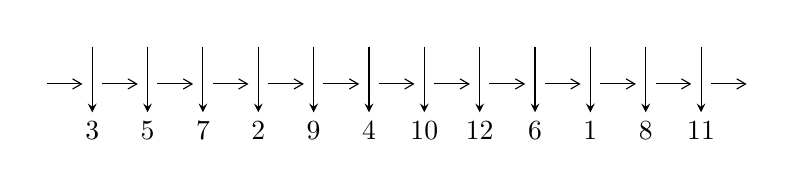
\begin{tikzpicture}[x=20pt, y=17pt]
	% nodes
	\node (C0) at (0, 0) {};
	\node (C1) at (1, 0) {};
	\node (C1U) at (1, +1) {};
	\node (C1D) at (1, -1) {3};

	\node (C2) at (2, 0) {};
	\node (C2U) at (2, +1) {};
	\node (C2D) at (2, -1) {5};

	\node (C3) at (3, 0) {};
	\node (C3U) at (3, +1) {};
	\node (C3D) at (3, -1) {7};

	\node (C4) at (4, 0) {};
	\node (C4U) at (4, +1) {};
	\node (C4D) at (4, -1) {2};

	\node (C5) at (5, 0) {};
	\node (C5U) at (5, +1) {};
	\node (C5D) at (5, -1) {9};

	\node (C6) at (6, 0) {};
	\node (C6U) at (6, +1) {};
	\node (C6D) at (6, -1) {4};

	\node (C7) at (7, 0) {};
	\node (C7U) at (7, +1) {};
	\node (C7D) at (7, -1) {10};

	\node (C8) at (8, 0) {};
	\node (C8U) at (8, +1) {};
	\node (C8D) at (8, -1) {12};

	\node (C9) at (9, 0) {};
	\node (C9U) at (9, +1) {};
	\node (C9D) at (9, -1) {6};

	\node (C10) at (10, 0) {};
	\node (C10U) at (10, +1) {};
	\node (C10D) at (10, -1) {1};

	\node (C11) at (11, 0) {};
	\node (C11U) at (11, +1) {};
	\node (C11D) at (11, -1) {8};

	\node (C12) at (12, 0) {};
	\node (C12U) at (12, +1) {};
	\node (C12D) at (12, -1) {11};
	\node (C13) at (13, 0) {};

	% arrows
	\draw[->,>={angle 60}]
	(C0) edge (C1) (C1) edge (C2) (C2) edge (C3) (C3) edge (C4) (C4) edge (C5) (C5) edge (C6) (C6) edge (C7) (C7) edge (C8) (C8) edge (C9) (C9) edge (C10) (C10) edge (C11) (C11) edge (C12) (C12) edge (C13) ;	\draw[->,>=stealth]
	(C1U) edge (C1D) (C2U) edge (C2D) (C3U) edge (C3D) (C4U) edge (C4D) (C5U) edge (C5D) (C6U) edge (C6D) (C7U) edge (C7D) (C8U) edge (C8D) (C9U) edge (C9D) (C10U) edge (C10D) (C11U) edge (C11D) (C12U) edge (C12D) ;
	\end{tikzpicture} \\
\hhline{~~} \\& 
\textbf{Solving Sequence} \\ \cline{2-2} 
 &
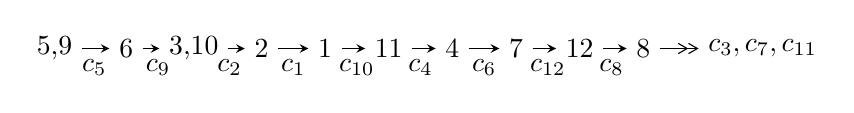
\begin{tikzpicture}[x=23pt, y=7pt]
	% node
	\node (A0) at (-1/8, 0) {5,9};
	\node (A1) at (1, 0) {6};
	\node (A2) at (33/16, 0) {3,10};
	\node (A3) at (25/8, 0) {2};
	\node (A4) at (33/8, 0) {1};
	\node (A5) at (41/8, 0) {11};
	\node (A6) at (49/8, 0) {4};
	\node (A7) at (57/8, 0) {7};
	\node (A8) at (65/8, 0) {12};
	\node (A9) at (73/8, 0) {8};
	\node (C1) at (1/2, -1) {$c_{5}$};
	\node (C2) at (3/2, -1) {$c_{9}$};
	\node (C3) at (21/8, -1) {$c_{2}$};
	\node (C4) at (29/8, -1) {$c_{1}$};
	\node (C5) at (37/8, -1) {$c_{10}$};
	\node (C6) at (45/8, -1) {$c_{4}$};
	\node (C7) at (53/8, -1) {$c_{6}$};
	\node (C8) at (61/8, -1) {$c_{12}$};
	\node (C9) at (69/8, -1) {$c_{8}$};
	\node (A10) at (11, 0) {$c_{3},c_{7},c_{11}$};

	% edge
	\draw[->,>=stealth]	
	(A0) edge (A1) (A1) edge (A2) (A2) edge (A3) (A3) edge (A4) (A4) edge (A5) (A5) edge (A6) (A6) edge (A7) (A7) edge (A8) (A8) edge (A9) ;
	\draw[->>,>={angle 60}]	
	(A9) edge (A10);
\end{tikzpicture} \\ 

\end{tabular} \\

\footnotetext{
The image of knot diagram is generated by the software ``\textbf{Draw programme}" developed by Andrew Bartholomew(\url{http://www.layer8.co.uk/maths/draw/index.htm\#Running-draw}), where we modified some parts for our purpose(\url{https://github.com/CATsTAILs/LinksPainter}).
}\phantom \\ \newline 
\centering \textbf{Ideals for irreducible components\footnotemark of $X_{\text{par}}$} 
 
\begin{align*}
I^u_{1}&=\langle 
1.12989\times10^{299} u^{117}-1.16841\times10^{300} u^{116}+\cdots+4.70875\times10^{301} b+1.53055\times10^{303},\\
\phantom{I^u_{1}}&\phantom{= \langle  }3.83387\times10^{299} u^{117}+8.89420\times10^{298} u^{116}+\cdots+2.35437\times10^{301} a-5.12301\times10^{302},\\
\phantom{I^u_{1}}&\phantom{= \langle  }u^{118}-2 u^{117}+\cdots+2560 u-512\rangle \\
I^u_{2}&=\langle 
b+1,\;2 u^7+3 u^6-5 u^5-7 u^4+4 u^3+3 u^2+a+4,\;u^8+u^7-3 u^6-2 u^5+3 u^4+2 u-1\rangle \\
\\
I^v_{1}&=\langle 
a,\;b- v-1,\;v^3+2 v^2+v+1\rangle \\
I^v_{2}&=\langle 
a,\;-89 v^5-27 v^4-1425 v^3+1434 v^2+80 b-1060 v+163,\;v^6+16 v^4-21 v^3+18 v^2-7 v+1\rangle \\
\end{align*}
\raggedright * 4 irreducible components of $\dim_{\mathbb{C}}=0$, with total 135 representations.\\
\footnotetext{All coefficients of polynomials are rational numbers. But the coefficients are sometimes approximated in decimal forms when there is not enough margin.}
\newpage
\renewcommand{\arraystretch}{1}
\centering \section*{I. $I^u_{1}= \langle 1.13\times10^{299} u^{117}-1.17\times10^{300} u^{116}+\cdots+4.71\times10^{301} b+1.53\times10^{303},\;3.83\times10^{299} u^{117}+8.89\times10^{298} u^{116}+\cdots+2.35\times10^{301} a-5.12\times10^{302},\;u^{118}-2 u^{117}+\cdots+2560 u-512 \rangle$}
\flushleft \textbf{(i) Arc colorings}\\
\begin{tabular}{m{7pt} m{180pt} m{7pt} m{180pt} }
\flushright $a_{5}=$&$\begin{pmatrix}1\\0\end{pmatrix}$ \\
\flushright $a_{9}=$&$\begin{pmatrix}0\\u\end{pmatrix}$ \\
\flushright $a_{6}=$&$\begin{pmatrix}1\\u^2\end{pmatrix}$ \\
\flushright $a_{3}=$&$\begin{pmatrix}-0.0162840 u^{117}-0.00377773 u^{116}+\cdots+7.00670 u+21.7596\\-0.00239956 u^{117}+0.0248136 u^{116}+\cdots+64.2202 u-32.5045\end{pmatrix}$ \\
\flushright $a_{10}=$&$\begin{pmatrix}- u\\- u^3+u\end{pmatrix}$ \\
\flushright $a_{2}=$&$\begin{pmatrix}-0.0186836 u^{117}+0.0210359 u^{116}+\cdots+71.2269 u-10.7449\\-0.00239956 u^{117}+0.0248136 u^{116}+\cdots+64.2202 u-32.5045\end{pmatrix}$ \\
\flushright $a_{1}=$&$\begin{pmatrix}0.239969 u^{117}-0.352060 u^{116}+\cdots-716.486 u+221.132\\-0.292188 u^{117}+0.424993 u^{116}+\cdots+866.378 u-258.873\end{pmatrix}$ \\
\flushright $a_{11}=$&$\begin{pmatrix}-0.131955 u^{117}+0.204289 u^{116}+\cdots+413.640 u-128.922\\0.221589 u^{117}-0.335927 u^{116}+\cdots-682.434 u+206.678\end{pmatrix}$ \\
\flushright $a_{4}=$&$\begin{pmatrix}0.0733908 u^{117}-0.115200 u^{116}+\cdots-209.169 u+71.7653\\-0.172469 u^{117}+0.223238 u^{116}+\cdots+440.130 u-109.957\end{pmatrix}$ \\
\flushright $a_{7}=$&$\begin{pmatrix}-0.0522189 u^{117}+0.0729326 u^{116}+\cdots+149.893 u-37.7416\\0.277615 u^{117}-0.398424 u^{116}+\cdots-812.461 u+242.743\end{pmatrix}$ \\
\flushright $a_{12}=$&$\begin{pmatrix}0.265862 u^{117}-0.404606 u^{116}+\cdots-827.746 u+260.201\\-0.364450 u^{117}+0.560905 u^{116}+\cdots+1155.73 u-356.859\end{pmatrix}$ \\
\flushright $a_{8}=$&$\begin{pmatrix}-0.116915 u^{117}+0.172605 u^{116}+\cdots+354.396 u-103.215\\0.331573 u^{117}-0.477354 u^{116}+\cdots-974.009 u+293.000\end{pmatrix}$\\&\end{tabular}
\flushleft \textbf{(ii) Obstruction class $= -1$}\\~\\
\flushleft \textbf{(iii) Cusp Shapes $= 1.80808 u^{117}-2.59255 u^{116}+\cdots-5062.88 u+1486.83$}\\~\\
\newpage\renewcommand{\arraystretch}{1}
\flushleft \textbf{(iv) u-Polynomials at the component}\newline \\
\begin{tabular}{m{50pt}|m{274pt}}
Crossings & \hspace{64pt}u-Polynomials at each crossing \\
\hline $$\begin{aligned}c_{1}\end{aligned}$$&$\begin{aligned}
&u^{118}+56 u^{117}+\cdots+165 u+1
\end{aligned}$\\
\hline $$\begin{aligned}c_{2},c_{4}\end{aligned}$$&$\begin{aligned}
&u^{118}-12 u^{117}+\cdots+13 u+1
\end{aligned}$\\
\hline $$\begin{aligned}c_{3},c_{6}\end{aligned}$$&$\begin{aligned}
&u^{118}-4 u^{117}+\cdots+1664 u-256
\end{aligned}$\\
\hline $$\begin{aligned}c_{5},c_{9}\end{aligned}$$&$\begin{aligned}
&u^{118}+2 u^{117}+\cdots-2560 u-512
\end{aligned}$\\
\hline $$\begin{aligned}c_{7}\end{aligned}$$&$\begin{aligned}
&u^{118}-5 u^{117}+\cdots-42339 u+2017
\end{aligned}$\\
\hline $$\begin{aligned}c_{8},c_{11}\end{aligned}$$&$\begin{aligned}
&u^{118}+5 u^{117}+\cdots+11 u+1
\end{aligned}$\\
\hline $$\begin{aligned}c_{10},c_{12}\end{aligned}$$&$\begin{aligned}
&u^{118}+39 u^{117}+\cdots-19 u+1
\end{aligned}$\\
\hline
\end{tabular}\\~\\
\newpage\renewcommand{\arraystretch}{1}
\flushleft \textbf{(v) Riley Polynomials at the component}\newline \\
\begin{tabular}{m{50pt}|m{274pt}}
Crossings & \hspace{64pt}Riley Polynomials at each crossing \\
\hline $$\begin{aligned}c_{1}\end{aligned}$$&$\begin{aligned}
&y^{118}+24 y^{117}+\cdots-12937 y+1
\end{aligned}$\\
\hline $$\begin{aligned}c_{2},c_{4}\end{aligned}$$&$\begin{aligned}
&y^{118}-56 y^{117}+\cdots-165 y+1
\end{aligned}$\\
\hline $$\begin{aligned}c_{3},c_{6}\end{aligned}$$&$\begin{aligned}
&y^{118}+60 y^{117}+\cdots-1228800 y+65536
\end{aligned}$\\
\hline $$\begin{aligned}c_{5},c_{9}\end{aligned}$$&$\begin{aligned}
&y^{118}-56 y^{117}+\cdots-9306112 y+262144
\end{aligned}$\\
\hline $$\begin{aligned}c_{7}\end{aligned}$$&$\begin{aligned}
&y^{118}-11 y^{117}+\cdots+141591059 y+4068289
\end{aligned}$\\
\hline $$\begin{aligned}c_{8},c_{11}\end{aligned}$$&$\begin{aligned}
&y^{118}-39 y^{117}+\cdots+19 y+1
\end{aligned}$\\
\hline $$\begin{aligned}c_{10},c_{12}\end{aligned}$$&$\begin{aligned}
&y^{118}+85 y^{117}+\cdots-157 y+1
\end{aligned}$\\
\hline
\end{tabular}\\~\\
\newpage\flushleft \textbf{(vi) Complex Volumes and Cusp Shapes}
$$\begin{array}{c|c|c}  
\text{Solutions to }I^u_{1}& \I (\text{vol} + \sqrt{-1}CS) & \text{Cusp shape}\\
 \hline 
\begin{aligned}
u &= -0.968041 + 0.257958 I \\
a &= -1.095610 + 0.036404 I \\
b &= -1.208900 - 0.211455 I\end{aligned}
 & -3.20568 + 0.98478 I & \phantom{-0.000000 } 0 \\ \hline\begin{aligned}
u &= -0.968041 - 0.257958 I \\
a &= -1.095610 - 0.036404 I \\
b &= -1.208900 + 0.211455 I\end{aligned}
 & -3.20568 - 0.98478 I & \phantom{-0.000000 } 0 \\ \hline\begin{aligned}
u &= \phantom{-}0.829247 + 0.549290 I \\
a &= -0.865086 - 0.372811 I \\
b &= \phantom{-}0.553838 - 0.724684 I\end{aligned}
 & \phantom{-}6.32463 + 3.26581 I & \phantom{-0.000000 } 0 \\ \hline\begin{aligned}
u &= \phantom{-}0.829247 - 0.549290 I \\
a &= -0.865086 + 0.372811 I \\
b &= \phantom{-}0.553838 + 0.724684 I\end{aligned}
 & \phantom{-}6.32463 - 3.26581 I & \phantom{-0.000000 } 0 \\ \hline\begin{aligned}
u &= -0.415238 + 0.916584 I \\
a &= \phantom{-}1.23962 + 1.28903 I \\
b &= -0.981130 - 0.446334 I\end{aligned}
 & \phantom{-}0.99666 - 5.77439 I & \phantom{-0.000000 } 0 \\ \hline\begin{aligned}
u &= -0.415238 - 0.916584 I \\
a &= \phantom{-}1.23962 - 1.28903 I \\
b &= -0.981130 + 0.446334 I\end{aligned}
 & \phantom{-}0.99666 + 5.77439 I & \phantom{-0.000000 } 0 \\ \hline\begin{aligned}
u &= \phantom{-}0.482135 + 0.901109 I \\
a &= \phantom{-}0.214333 - 1.168030 I \\
b &= \phantom{-}0.447969 + 0.621910 I\end{aligned}
 & \phantom{-}0.099568 + 0.954515 I & \phantom{-0.000000 } 0 \\ \hline\begin{aligned}
u &= \phantom{-}0.482135 - 0.901109 I \\
a &= \phantom{-}0.214333 + 1.168030 I \\
b &= \phantom{-}0.447969 - 0.621910 I\end{aligned}
 & \phantom{-}0.099568 - 0.954515 I & \phantom{-0.000000 } 0 \\ \hline\begin{aligned}
u &= \phantom{-}0.249986 + 0.944644 I \\
a &= -0.120617 - 0.867968 I \\
b &= \phantom{-}0.793060 + 0.496364 I\end{aligned}
 & \phantom{-}1.78559 - 4.11675 I & \phantom{-0.000000 } 0 \\ \hline\begin{aligned}
u &= \phantom{-}0.249986 - 0.944644 I \\
a &= -0.120617 + 0.867968 I \\
b &= \phantom{-}0.793060 - 0.496364 I\end{aligned}
 & \phantom{-}1.78559 + 4.11675 I & \phantom{-0.000000 } 0\\
 \hline 
 \end{array}$$\newpage$$\begin{array}{c|c|c}  
\text{Solutions to }I^u_{1}& \I (\text{vol} + \sqrt{-1}CS) & \text{Cusp shape}\\
 \hline 
\begin{aligned}
u &= -0.799310 + 0.561370 I \\
a &= -0.196431 + 1.338860 I \\
b &= \phantom{-}0.715155 - 0.892572 I\end{aligned}
 & \phantom{-}6.93896 + 1.81575 I & \phantom{-0.000000 } 0 \\ \hline\begin{aligned}
u &= -0.799310 - 0.561370 I \\
a &= -0.196431 - 1.338860 I \\
b &= \phantom{-}0.715155 + 0.892572 I\end{aligned}
 & \phantom{-}6.93896 - 1.81575 I & \phantom{-0.000000 } 0 \\ \hline\begin{aligned}
u &= \phantom{-}0.843723 + 0.487342 I \\
a &= -0.237848 - 1.342180 I \\
b &= \phantom{-}0.748925 + 0.908083 I\end{aligned}
 & \phantom{-}6.30583 - 7.44643 I & \phantom{-0.000000 } 0 \\ \hline\begin{aligned}
u &= \phantom{-}0.843723 - 0.487342 I \\
a &= -0.237848 + 1.342180 I \\
b &= \phantom{-}0.748925 - 0.908083 I\end{aligned}
 & \phantom{-}6.30583 + 7.44643 I & \phantom{-0.000000 } 0 \\ \hline\begin{aligned}
u &= \phantom{-}0.478089 + 0.846590 I \\
a &= \phantom{-}1.25380 - 1.23453 I \\
b &= -0.930674 + 0.453400 I\end{aligned}
 & \phantom{-}1.68529 + 0.26296 I & \phantom{-0.000000 } 0 \\ \hline\begin{aligned}
u &= \phantom{-}0.478089 - 0.846590 I \\
a &= \phantom{-}1.25380 + 1.23453 I \\
b &= -0.930674 - 0.453400 I\end{aligned}
 & \phantom{-}1.68529 - 0.26296 I & \phantom{-0.000000 } 0 \\ \hline\begin{aligned}
u &= -0.853323 + 0.583684 I \\
a &= -0.906160 + 0.157216 I \\
b &= \phantom{-}0.528021 + 0.758724 I\end{aligned}
 & \phantom{-}6.75979 + 2.72376 I & \phantom{-0.000000 } 0 \\ \hline\begin{aligned}
u &= -0.853323 - 0.583684 I \\
a &= -0.906160 - 0.157216 I \\
b &= \phantom{-}0.528021 - 0.758724 I\end{aligned}
 & \phantom{-}6.75979 - 2.72376 I & \phantom{-0.000000 } 0 \\ \hline\begin{aligned}
u &= \phantom{-}0.972715 + 0.354059 I \\
a &= \phantom{-}1.75870 - 1.27137 I \\
b &= \phantom{-}1.028880 + 0.606831 I\end{aligned}
 & \phantom{-}4.90526 - 1.82621 I & \phantom{-0.000000 } 0 \\ \hline\begin{aligned}
u &= \phantom{-}0.972715 - 0.354059 I \\
a &= \phantom{-}1.75870 + 1.27137 I \\
b &= \phantom{-}1.028880 - 0.606831 I\end{aligned}
 & \phantom{-}4.90526 + 1.82621 I & \phantom{-0.000000 } 0\\
 \hline 
 \end{array}$$\newpage$$\begin{array}{c|c|c}  
\text{Solutions to }I^u_{1}& \I (\text{vol} + \sqrt{-1}CS) & \text{Cusp shape}\\
 \hline 
\begin{aligned}
u &= -0.985328 + 0.420063 I \\
a &= \phantom{-}1.57530 + 1.48448 I \\
b &= \phantom{-}1.049240 - 0.617926 I\end{aligned}
 & \phantom{-}5.20076 + 7.94162 I & \phantom{-0.000000 } 0 \\ \hline\begin{aligned}
u &= -0.985328 - 0.420063 I \\
a &= \phantom{-}1.57530 - 1.48448 I \\
b &= \phantom{-}1.049240 + 0.617926 I\end{aligned}
 & \phantom{-}5.20076 - 7.94162 I & \phantom{-0.000000 } 0 \\ \hline\begin{aligned}
u &= -0.520970 + 0.762195 I \\
a &= -0.023391 + 1.189300 I \\
b &= \phantom{-}0.622197 - 0.716300 I\end{aligned}
 & \phantom{-}3.44231 + 1.13448 I & \phantom{-0.000000 } 0 \\ \hline\begin{aligned}
u &= -0.520970 - 0.762195 I \\
a &= -0.023391 - 1.189300 I \\
b &= \phantom{-}0.622197 + 0.716300 I\end{aligned}
 & \phantom{-}3.44231 - 1.13448 I & \phantom{-0.000000 } 0 \\ \hline\begin{aligned}
u &= \phantom{-}1.016500 + 0.411656 I \\
a &= -0.57750 + 1.92773 I \\
b &= -1.025370 - 0.473801 I\end{aligned}
 & -2.56259 - 3.40175 I & \phantom{-0.000000 } 0 \\ \hline\begin{aligned}
u &= \phantom{-}1.016500 - 0.411656 I \\
a &= -0.57750 - 1.92773 I \\
b &= -1.025370 + 0.473801 I\end{aligned}
 & -2.56259 + 3.40175 I & \phantom{-0.000000 } 0 \\ \hline\begin{aligned}
u &= -1.068630 + 0.250244 I \\
a &= \phantom{-}0.732536 + 0.841832 I \\
b &= -0.410454 - 0.655638 I\end{aligned}
 & -4.72278 + 0.90000 I & \phantom{-0.000000 } 0 \\ \hline\begin{aligned}
u &= -1.068630 - 0.250244 I \\
a &= \phantom{-}0.732536 - 0.841832 I \\
b &= -0.410454 + 0.655638 I\end{aligned}
 & -4.72278 - 0.90000 I & \phantom{-0.000000 } 0 \\ \hline\begin{aligned}
u &= \phantom{-}0.990053 + 0.499135 I \\
a &= \phantom{-}0.921702 - 0.978841 I \\
b &= -0.598504 + 0.641847 I\end{aligned}
 & \phantom{-}0.972070 - 0.862575 I & \phantom{-0.000000 } 0 \\ \hline\begin{aligned}
u &= \phantom{-}0.990053 - 0.499135 I \\
a &= \phantom{-}0.921702 + 0.978841 I \\
b &= -0.598504 - 0.641847 I\end{aligned}
 & \phantom{-}0.972070 + 0.862575 I & \phantom{-0.000000 } 0\\
 \hline 
 \end{array}$$\newpage$$\begin{array}{c|c|c}  
\text{Solutions to }I^u_{1}& \I (\text{vol} + \sqrt{-1}CS) & \text{Cusp shape}\\
 \hline 
\begin{aligned}
u &= -0.243622 + 0.854934 I \\
a &= -0.381125 - 0.936603 I \\
b &= \phantom{-}0.975067 + 0.617838 I\end{aligned}
 & \phantom{-}2.38535 - 3.97142 I & \phantom{-0.000000 } 0 \\ \hline\begin{aligned}
u &= -0.243622 - 0.854934 I \\
a &= -0.381125 + 0.936603 I \\
b &= \phantom{-}0.975067 - 0.617838 I\end{aligned}
 & \phantom{-}2.38535 + 3.97142 I & \phantom{-0.000000 } 0 \\ \hline\begin{aligned}
u &= -1.114060 + 0.037982 I \\
a &= \phantom{-}0.446073 - 0.685881 I \\
b &= -0.171434 + 0.680603 I\end{aligned}
 & -1.57653 + 4.72128 I & \phantom{-0.000000 } 0 \\ \hline\begin{aligned}
u &= -1.114060 - 0.037982 I \\
a &= \phantom{-}0.446073 + 0.685881 I \\
b &= -0.171434 - 0.680603 I\end{aligned}
 & -1.57653 - 4.72128 I & \phantom{-0.000000 } 0 \\ \hline\begin{aligned}
u &= \phantom{-}1.027390 + 0.442691 I \\
a &= -0.166893 + 0.306639 I \\
b &= \phantom{-}0.252493 - 0.709156 I\end{aligned}
 & -0.506538 - 0.358617 I & \phantom{-0.000000 } 0 \\ \hline\begin{aligned}
u &= \phantom{-}1.027390 - 0.442691 I \\
a &= -0.166893 - 0.306639 I \\
b &= \phantom{-}0.252493 + 0.709156 I\end{aligned}
 & -0.506538 + 0.358617 I & \phantom{-0.000000 } 0 \\ \hline\begin{aligned}
u &= \phantom{-}0.861028 + 0.151410 I \\
a &= \phantom{-}0.522984 + 0.294298 I \\
b &= -0.049918 - 0.430497 I\end{aligned}
 & -0.628133 - 0.111774 I & \phantom{-0.000000 } 0 \\ \hline\begin{aligned}
u &= \phantom{-}0.861028 - 0.151410 I \\
a &= \phantom{-}0.522984 - 0.294298 I \\
b &= -0.049918 + 0.430497 I\end{aligned}
 & -0.628133 + 0.111774 I & \phantom{-0.000000 } 0 \\ \hline\begin{aligned}
u &= -0.614884 + 0.943203 I \\
a &= \phantom{-}0.117724 + 1.369210 I \\
b &= \phantom{-}0.448785 - 0.808428 I\end{aligned}
 & \phantom{-}6.24801 - 0.38665 I & \phantom{-0.000000 } 0 \\ \hline\begin{aligned}
u &= -0.614884 - 0.943203 I \\
a &= \phantom{-}0.117724 - 1.369210 I \\
b &= \phantom{-}0.448785 + 0.808428 I\end{aligned}
 & \phantom{-}6.24801 + 0.38665 I & \phantom{-0.000000 } 0\\
 \hline 
 \end{array}$$\newpage$$\begin{array}{c|c|c}  
\text{Solutions to }I^u_{1}& \I (\text{vol} + \sqrt{-1}CS) & \text{Cusp shape}\\
 \hline 
\begin{aligned}
u &= \phantom{-}0.031010 + 1.128990 I \\
a &= -0.316506 + 0.783217 I \\
b &= \phantom{-}0.963150 - 0.484891 I\end{aligned}
 & \phantom{-}1.155310 - 0.197698 I & \phantom{-0.000000 } 0 \\ \hline\begin{aligned}
u &= \phantom{-}0.031010 - 1.128990 I \\
a &= -0.316506 - 0.783217 I \\
b &= \phantom{-}0.963150 + 0.484891 I\end{aligned}
 & \phantom{-}1.155310 + 0.197698 I & \phantom{-0.000000 } 0 \\ \hline\begin{aligned}
u &= \phantom{-}0.268922 + 0.827360 I \\
a &= \phantom{-}0.72388 + 1.84885 I \\
b &= -1.168050 - 0.164940 I\end{aligned}
 & \phantom{-}0.29288 + 3.57986 I & \phantom{-0.000000 } 0 \\ \hline\begin{aligned}
u &= \phantom{-}0.268922 - 0.827360 I \\
a &= \phantom{-}0.72388 - 1.84885 I \\
b &= -1.168050 + 0.164940 I\end{aligned}
 & \phantom{-}0.29288 - 3.57986 I & \phantom{-0.000000 } 0 \\ \hline\begin{aligned}
u &= \phantom{-}0.590336 + 0.982576 I \\
a &= \phantom{-}0.167145 - 1.387410 I \\
b &= \phantom{-}0.403326 + 0.803323 I\end{aligned}
 & \phantom{-}5.42643 + 6.09310 I & \phantom{-0.000000 } 0 \\ \hline\begin{aligned}
u &= \phantom{-}0.590336 - 0.982576 I \\
a &= \phantom{-}0.167145 + 1.387410 I \\
b &= \phantom{-}0.403326 - 0.803323 I\end{aligned}
 & \phantom{-}5.42643 - 6.09310 I & \phantom{-0.000000 } 0 \\ \hline\begin{aligned}
u &= \phantom{-}0.777956 + 0.330194 I \\
a &= -0.458677 + 1.167580 I \\
b &= \phantom{-}0.981131 - 0.822526 I\end{aligned}
 & \phantom{-}5.61296 - 1.12841 I & \phantom{-0.000000 } 0 \\ \hline\begin{aligned}
u &= \phantom{-}0.777956 - 0.330194 I \\
a &= -0.458677 - 1.167580 I \\
b &= \phantom{-}0.981131 + 0.822526 I\end{aligned}
 & \phantom{-}5.61296 + 1.12841 I & \phantom{-0.000000 } 0 \\ \hline\begin{aligned}
u &= -0.718794 + 0.438941 I \\
a &= -0.466394 - 1.130240 I \\
b &= \phantom{-}0.996581 + 0.793604 I\end{aligned}
 & \phantom{-}6.09920 - 4.36602 I & \phantom{-0.000000 } 0 \\ \hline\begin{aligned}
u &= -0.718794 - 0.438941 I \\
a &= -0.466394 + 1.130240 I \\
b &= \phantom{-}0.996581 - 0.793604 I\end{aligned}
 & \phantom{-}6.09920 + 4.36602 I & \phantom{-0.000000 } 0\\
 \hline 
 \end{array}$$\newpage$$\begin{array}{c|c|c}  
\text{Solutions to }I^u_{1}& \I (\text{vol} + \sqrt{-1}CS) & \text{Cusp shape}\\
 \hline 
\begin{aligned}
u &= -1.139670 + 0.233858 I \\
a &= -0.64291 - 1.42563 I \\
b &= -1.125200 + 0.435963 I\end{aligned}
 & -4.44670 - 0.52239 I & \phantom{-0.000000 } 0 \\ \hline\begin{aligned}
u &= -1.139670 - 0.233858 I \\
a &= -0.64291 + 1.42563 I \\
b &= -1.125200 - 0.435963 I\end{aligned}
 & -4.44670 + 0.52239 I & \phantom{-0.000000 } 0 \\ \hline\begin{aligned}
u &= \phantom{-}1.165730 + 0.117225 I \\
a &= -0.711644 - 0.603236 I \\
b &= -1.233320 + 0.315637 I\end{aligned}
 & -4.75315 + 3.18722 I & \phantom{-0.000000 } 0 \\ \hline\begin{aligned}
u &= \phantom{-}1.165730 - 0.117225 I \\
a &= -0.711644 + 0.603236 I \\
b &= -1.233320 - 0.315637 I\end{aligned}
 & -4.75315 - 3.18722 I & \phantom{-0.000000 } 0 \\ \hline\begin{aligned}
u &= -0.377624 + 0.735819 I \\
a &= \phantom{-}0.37330 - 1.98922 I \\
b &= -1.174320 + 0.104126 I\end{aligned}
 & \phantom{-}0.77652 + 1.81636 I & -12.00000 + 0. I\phantom{ +0.000000I} \\ \hline\begin{aligned}
u &= -0.377624 - 0.735819 I \\
a &= \phantom{-}0.37330 + 1.98922 I \\
b &= -1.174320 - 0.104126 I\end{aligned}
 & \phantom{-}0.77652 - 1.81636 I & -12.00000 + 0. I\phantom{ +0.000000I} \\ \hline\begin{aligned}
u &= -1.072760 + 0.484709 I \\
a &= \phantom{-}0.860812 + 1.003010 I \\
b &= -0.574193 - 0.692752 I\end{aligned}
 & \phantom{-}0.05864 + 6.41739 I & \phantom{-0.000000 } 0 \\ \hline\begin{aligned}
u &= -1.072760 - 0.484709 I \\
a &= \phantom{-}0.860812 - 1.003010 I \\
b &= -0.574193 + 0.692752 I\end{aligned}
 & \phantom{-}0.05864 - 6.41739 I & \phantom{-0.000000 } 0 \\ \hline\begin{aligned}
u &= \phantom{-}0.336930 + 1.138880 I \\
a &= -0.462918 + 0.832786 I \\
b &= \phantom{-}1.062340 - 0.556419 I\end{aligned}
 & -1.69323 + 5.63066 I & \phantom{-0.000000 } 0 \\ \hline\begin{aligned}
u &= \phantom{-}0.336930 - 1.138880 I \\
a &= -0.462918 - 0.832786 I \\
b &= \phantom{-}1.062340 + 0.556419 I\end{aligned}
 & -1.69323 - 5.63066 I & \phantom{-0.000000 } 0\\
 \hline 
 \end{array}$$\newpage$$\begin{array}{c|c|c}  
\text{Solutions to }I^u_{1}& \I (\text{vol} + \sqrt{-1}CS) & \text{Cusp shape}\\
 \hline 
\begin{aligned}
u &= -0.537139 + 1.064810 I \\
a &= -0.528088 - 0.903093 I \\
b &= \phantom{-}1.097750 + 0.625048 I\end{aligned}
 & \phantom{-}4.31525 - 5.75325 I & \phantom{-0.000000 } 0 \\ \hline\begin{aligned}
u &= -0.537139 - 1.064810 I \\
a &= -0.528088 + 0.903093 I \\
b &= \phantom{-}1.097750 - 0.625048 I\end{aligned}
 & \phantom{-}4.31525 + 5.75325 I & \phantom{-0.000000 } 0 \\ \hline\begin{aligned}
u &= -1.037560 + 0.589522 I \\
a &= -0.548931 - 0.411253 I \\
b &= \phantom{-}0.357729 + 0.832116 I\end{aligned}
 & \phantom{-}1.88903 + 3.97132 I & \phantom{-0.000000 } 0 \\ \hline\begin{aligned}
u &= -1.037560 - 0.589522 I \\
a &= -0.548931 + 0.411253 I \\
b &= \phantom{-}0.357729 - 0.832116 I\end{aligned}
 & \phantom{-}1.88903 - 3.97132 I & \phantom{-0.000000 } 0 \\ \hline\begin{aligned}
u &= -0.132287 + 0.795513 I \\
a &= \phantom{-}1.35850 + 1.53988 I \\
b &= -1.023230 - 0.290062 I\end{aligned}
 & -3.52217 - 0.96416 I & -19.6651 + 0. I\phantom{ +0.000000I} \\ \hline\begin{aligned}
u &= -0.132287 - 0.795513 I \\
a &= \phantom{-}1.35850 - 1.53988 I \\
b &= -1.023230 + 0.290062 I\end{aligned}
 & -3.52217 + 0.96416 I & -19.6651 + 0. I\phantom{ +0.000000I} \\ \hline\begin{aligned}
u &= -1.085610 + 0.543986 I \\
a &= -0.356479 - 0.308822 I \\
b &= -1.327980 - 0.156554 I\end{aligned}
 & -1.30186 + 2.99365 I & \phantom{-0.000000 } 0 \\ \hline\begin{aligned}
u &= -1.085610 - 0.543986 I \\
a &= -0.356479 + 0.308822 I \\
b &= -1.327980 + 0.156554 I\end{aligned}
 & -1.30186 - 2.99365 I & \phantom{-0.000000 } 0 \\ \hline\begin{aligned}
u &= \phantom{-}1.167610 + 0.373716 I \\
a &= -0.483262 - 0.069876 I \\
b &= -1.305780 + 0.232105 I\end{aligned}
 & -7.40438 - 2.81707 I & \phantom{-0.000000 } 0 \\ \hline\begin{aligned}
u &= \phantom{-}1.167610 - 0.373716 I \\
a &= -0.483262 + 0.069876 I \\
b &= -1.305780 - 0.232105 I\end{aligned}
 & -7.40438 + 2.81707 I & \phantom{-0.000000 } 0\\
 \hline 
 \end{array}$$\newpage$$\begin{array}{c|c|c}  
\text{Solutions to }I^u_{1}& \I (\text{vol} + \sqrt{-1}CS) & \text{Cusp shape}\\
 \hline 
\begin{aligned}
u &= \phantom{-}0.540828 + 1.135790 I \\
a &= -0.544870 + 0.876987 I \\
b &= \phantom{-}1.116380 - 0.608106 I\end{aligned}
 & \phantom{-}3.30849 + 11.38200 I & \phantom{-0.000000 } 0 \\ \hline\begin{aligned}
u &= \phantom{-}0.540828 - 1.135790 I \\
a &= -0.544870 - 0.876987 I \\
b &= \phantom{-}1.116380 + 0.608106 I\end{aligned}
 & \phantom{-}3.30849 - 11.38200 I & \phantom{-0.000000 } 0 \\ \hline\begin{aligned}
u &= -1.174780 + 0.476913 I \\
a &= -0.28290 - 1.74882 I \\
b &= -1.074940 + 0.543544 I\end{aligned}
 & -6.67400 + 5.57881 I & \phantom{-0.000000 } 0 \\ \hline\begin{aligned}
u &= -1.174780 - 0.476913 I \\
a &= -0.28290 + 1.74882 I \\
b &= -1.074940 - 0.543544 I\end{aligned}
 & -6.67400 - 5.57881 I & \phantom{-0.000000 } 0 \\ \hline\begin{aligned}
u &= \phantom{-}1.110890 + 0.615385 I \\
a &= -0.14456 + 1.95078 I \\
b &= -1.013080 - 0.587449 I\end{aligned}
 & -0.28581 - 5.70221 I & \phantom{-0.000000 } 0 \\ \hline\begin{aligned}
u &= \phantom{-}1.110890 - 0.615385 I \\
a &= -0.14456 - 1.95078 I \\
b &= -1.013080 + 0.587449 I\end{aligned}
 & -0.28581 + 5.70221 I & \phantom{-0.000000 } 0 \\ \hline\begin{aligned}
u &= \phantom{-}1.150860 + 0.554359 I \\
a &= -0.260357 + 0.219493 I \\
b &= -1.350640 + 0.171559 I\end{aligned}
 & -2.33167 - 8.63976 I & \phantom{-0.000000 } 0 \\ \hline\begin{aligned}
u &= \phantom{-}1.150860 - 0.554359 I \\
a &= -0.260357 - 0.219493 I \\
b &= -1.350640 - 0.171559 I\end{aligned}
 & -2.33167 + 8.63976 I & \phantom{-0.000000 } 0 \\ \hline\begin{aligned}
u &= \phantom{-}0.557305 + 0.449357 I \\
a &= -0.51930 + 3.80205 I \\
b &= -0.801649 - 0.340065 I\end{aligned}
 & \phantom{-}2.29990 - 3.21991 I & -11.6454 + 9.3303 I \\ \hline\begin{aligned}
u &= \phantom{-}0.557305 - 0.449357 I \\
a &= -0.51930 - 3.80205 I \\
b &= -0.801649 + 0.340065 I\end{aligned}
 & \phantom{-}2.29990 + 3.21991 I & -11.6454 - 9.3303 I\\
 \hline 
 \end{array}$$\newpage$$\begin{array}{c|c|c}  
\text{Solutions to }I^u_{1}& \I (\text{vol} + \sqrt{-1}CS) & \text{Cusp shape}\\
 \hline 
\begin{aligned}
u &= \phantom{-}1.141930 + 0.609772 I \\
a &= -0.486454 + 0.645626 I \\
b &= \phantom{-}0.299791 - 0.906005 I\end{aligned}
 & -2.05151 - 6.52131 I & \phantom{-0.000000 } 0 \\ \hline\begin{aligned}
u &= \phantom{-}1.141930 - 0.609772 I \\
a &= -0.486454 - 0.645626 I \\
b &= \phantom{-}0.299791 + 0.906005 I\end{aligned}
 & -2.05151 + 6.52131 I & \phantom{-0.000000 } 0 \\ \hline\begin{aligned}
u &= -1.106120 + 0.710751 I \\
a &= -0.695103 - 0.696708 I \\
b &= \phantom{-}0.373079 + 0.947396 I\end{aligned}
 & \phantom{-}4.66095 + 6.47958 I & \phantom{-0.000000 } 0 \\ \hline\begin{aligned}
u &= -1.106120 - 0.710751 I \\
a &= -0.695103 + 0.696708 I \\
b &= \phantom{-}0.373079 - 0.947396 I\end{aligned}
 & \phantom{-}4.66095 - 6.47958 I & \phantom{-0.000000 } 0 \\ \hline\begin{aligned}
u &= -1.160330 + 0.627826 I \\
a &= -0.09864 - 1.89218 I \\
b &= -1.031920 + 0.604757 I\end{aligned}
 & -1.32480 + 11.44640 I & \phantom{-0.000000 } 0 \\ \hline\begin{aligned}
u &= -1.160330 - 0.627826 I \\
a &= -0.09864 + 1.89218 I \\
b &= -1.031920 - 0.604757 I\end{aligned}
 & -1.32480 - 11.44640 I & \phantom{-0.000000 } 0 \\ \hline\begin{aligned}
u &= -1.197040 + 0.583092 I \\
a &= \phantom{-}0.75573 + 1.45880 I \\
b &= \phantom{-}1.142950 - 0.603629 I\end{aligned}
 & -0.44954 + 9.31105 I & \phantom{-0.000000 } 0 \\ \hline\begin{aligned}
u &= -1.197040 - 0.583092 I \\
a &= \phantom{-}0.75573 - 1.45880 I \\
b &= \phantom{-}1.142950 + 0.603629 I\end{aligned}
 & -0.44954 - 9.31105 I & \phantom{-0.000000 } 0 \\ \hline\begin{aligned}
u &= \phantom{-}1.334630 + 0.023307 I \\
a &= \phantom{-}0.778731 + 0.175399 I \\
b &= \phantom{-}1.001030 - 0.399951 I\end{aligned}
 & -3.08028 + 2.84861 I & \phantom{-0.000000 } 0 \\ \hline\begin{aligned}
u &= \phantom{-}1.334630 - 0.023307 I \\
a &= \phantom{-}0.778731 - 0.175399 I \\
b &= \phantom{-}1.001030 + 0.399951 I\end{aligned}
 & -3.08028 - 2.84861 I & \phantom{-0.000000 } 0\\
 \hline 
 \end{array}$$\newpage$$\begin{array}{c|c|c}  
\text{Solutions to }I^u_{1}& \I (\text{vol} + \sqrt{-1}CS) & \text{Cusp shape}\\
 \hline 
\begin{aligned}
u &= \phantom{-}1.138450 + 0.719642 I \\
a &= -0.667790 + 0.755929 I \\
b &= \phantom{-}0.358664 - 0.967401 I\end{aligned}
 & \phantom{-}3.65490 - 12.33480 I & \phantom{-0.000000 } 0 \\ \hline\begin{aligned}
u &= \phantom{-}1.138450 - 0.719642 I \\
a &= -0.667790 - 0.755929 I \\
b &= \phantom{-}0.358664 + 0.967401 I\end{aligned}
 & \phantom{-}3.65490 + 12.33480 I & \phantom{-0.000000 } 0 \\ \hline\begin{aligned}
u &= \phantom{-}1.276910 + 0.487951 I \\
a &= \phantom{-}0.749851 - 1.177460 I \\
b &= \phantom{-}1.139720 + 0.557439 I\end{aligned}
 & -3.01548 - 5.22865 I & \phantom{-0.000000 } 0 \\ \hline\begin{aligned}
u &= \phantom{-}1.276910 - 0.487951 I \\
a &= \phantom{-}0.749851 + 1.177460 I \\
b &= \phantom{-}1.139720 - 0.557439 I\end{aligned}
 & -3.01548 + 5.22865 I & \phantom{-0.000000 } 0 \\ \hline\begin{aligned}
u &= \phantom{-}1.333150 + 0.335645 I \\
a &= \phantom{-}0.532133 - 0.147238 I \\
b &= \phantom{-}0.902286 - 0.299866 I\end{aligned}
 & -2.37987 - 0.21837 I & \phantom{-0.000000 } 0 \\ \hline\begin{aligned}
u &= \phantom{-}1.333150 - 0.335645 I \\
a &= \phantom{-}0.532133 + 0.147238 I \\
b &= \phantom{-}0.902286 + 0.299866 I\end{aligned}
 & -2.37987 + 0.21837 I & \phantom{-0.000000 } 0 \\ \hline\begin{aligned}
u &= \phantom{-}0.606553 + 0.136516 I \\
a &= -0.323621 - 1.210050 I \\
b &= \phantom{-}0.858468 + 0.822607 I\end{aligned}
 & \phantom{-}1.55699 - 3.04585 I & -22.2897 + 7.2245 I \\ \hline\begin{aligned}
u &= \phantom{-}0.606553 - 0.136516 I \\
a &= -0.323621 + 1.210050 I \\
b &= \phantom{-}0.858468 - 0.822607 I\end{aligned}
 & \phantom{-}1.55699 + 3.04585 I & -22.2897 - 7.2245 I \\ \hline\begin{aligned}
u &= -1.194310 + 0.735932 I \\
a &= \phantom{-}0.49361 + 1.67781 I \\
b &= \phantom{-}1.179130 - 0.645250 I\end{aligned}
 & \phantom{-}2.20206 + 12.28150 I & \phantom{-0.000000 } 0 \\ \hline\begin{aligned}
u &= -1.194310 - 0.735932 I \\
a &= \phantom{-}0.49361 - 1.67781 I \\
b &= \phantom{-}1.179130 + 0.645250 I\end{aligned}
 & \phantom{-}2.20206 - 12.28150 I & \phantom{-0.000000 } 0\\
 \hline 
 \end{array}$$\newpage$$\begin{array}{c|c|c}  
\text{Solutions to }I^u_{1}& \I (\text{vol} + \sqrt{-1}CS) & \text{Cusp shape}\\
 \hline 
\begin{aligned}
u &= \phantom{-}0.032258 + 0.593857 I \\
a &= \phantom{-}1.85959 - 0.38959 I \\
b &= -0.164637 + 0.077592 I\end{aligned}
 & \phantom{-}2.37401 - 2.69643 I & -3.59687 + 2.70387 I \\ \hline\begin{aligned}
u &= \phantom{-}0.032258 - 0.593857 I \\
a &= \phantom{-}1.85959 + 0.38959 I \\
b &= -0.164637 - 0.077592 I\end{aligned}
 & \phantom{-}2.37401 + 2.69643 I & -3.59687 - 2.70387 I \\ \hline\begin{aligned}
u &= -0.453797 + 0.354290 I \\
a &= -0.97607 - 5.19517 I \\
b &= -0.790637 + 0.250799 I\end{aligned}
 & \phantom{-}2.05724 - 2.52902 I & -14.1044 - 7.2590 I \\ \hline\begin{aligned}
u &= -0.453797 - 0.354290 I \\
a &= -0.97607 + 5.19517 I \\
b &= -0.790637 - 0.250799 I\end{aligned}
 & \phantom{-}2.05724 + 2.52902 I & -14.1044 + 7.2590 I \\ \hline\begin{aligned}
u &= \phantom{-}1.27377 + 0.66046 I \\
a &= \phantom{-}0.51916 - 1.45394 I \\
b &= \phantom{-}1.182920 + 0.605604 I\end{aligned}
 & -4.71019 - 12.03970 I & \phantom{-0.000000 } 0 \\ \hline\begin{aligned}
u &= \phantom{-}1.27377 - 0.66046 I \\
a &= \phantom{-}0.51916 + 1.45394 I \\
b &= \phantom{-}1.182920 - 0.605604 I\end{aligned}
 & -4.71019 + 12.03970 I & \phantom{-0.000000 } 0 \\ \hline\begin{aligned}
u &= \phantom{-}1.22016 + 0.76098 I \\
a &= \phantom{-}0.42193 - 1.65996 I \\
b &= \phantom{-}1.192000 + 0.646097 I\end{aligned}
 & \phantom{-}1.1052 - 18.1923 I & \phantom{-0.000000 } 0 \\ \hline\begin{aligned}
u &= \phantom{-}1.22016 - 0.76098 I \\
a &= \phantom{-}0.42193 + 1.65996 I \\
b &= \phantom{-}1.192000 - 0.646097 I\end{aligned}
 & \phantom{-}1.1052 + 18.1923 I & \phantom{-0.000000 } 0 \\ \hline\begin{aligned}
u &= -1.44666 + 0.06158 I \\
a &= \phantom{-}0.640057 + 0.341446 I \\
b &= \phantom{-}1.060440 - 0.388230 I\end{aligned}
 & -4.87122 + 7.86476 I & \phantom{-0.000000 } 0 \\ \hline\begin{aligned}
u &= -1.44666 - 0.06158 I \\
a &= \phantom{-}0.640057 - 0.341446 I \\
b &= \phantom{-}1.060440 + 0.388230 I\end{aligned}
 & -4.87122 - 7.86476 I & \phantom{-0.000000 } 0\\
 \hline 
 \end{array}$$\newpage$$\begin{array}{c|c|c}  
\text{Solutions to }I^u_{1}& \I (\text{vol} + \sqrt{-1}CS) & \text{Cusp shape}\\
 \hline 
\begin{aligned}
u &= \phantom{-}0.524803\phantom{ +0.000000I} \\
a &= \phantom{-}0.867240\phantom{ +0.000000I} \\
b &= -0.0932121\phantom{ +0.000000I}\end{aligned}
 & -0.780063\phantom{ +0.000000I} & -12.4920\phantom{ +0.000000I} \\ \hline\begin{aligned}
u &= -1.42325 + 0.40242 I \\
a &= \phantom{-}0.440992 + 0.117684 I \\
b &= \phantom{-}0.917187 + 0.253600 I\end{aligned}
 & -3.84346 + 5.72004 I & \phantom{-0.000000 } 0 \\ \hline\begin{aligned}
u &= -1.42325 - 0.40242 I \\
a &= \phantom{-}0.440992 - 0.117684 I \\
b &= \phantom{-}0.917187 - 0.253600 I\end{aligned}
 & -3.84346 - 5.72004 I & \phantom{-0.000000 } 0 \\ \hline\begin{aligned}
u &= -1.47689 + 0.17377 I \\
a &= \phantom{-}0.528339 - 0.069385 I \\
b &= \phantom{-}0.995495 + 0.310761 I\end{aligned}
 & -8.36236 - 1.00432 I & \phantom{-0.000000 } 0 \\ \hline\begin{aligned}
u &= -1.47689 - 0.17377 I \\
a &= \phantom{-}0.528339 + 0.069385 I \\
b &= \phantom{-}0.995495 - 0.310761 I\end{aligned}
 & -8.36236 + 1.00432 I & \phantom{-0.000000 } 0 \\ \hline\begin{aligned}
u &= \phantom{-}0.408179 + 0.268119 I \\
a &= \phantom{-}1.59911 - 0.55685 I \\
b &= -0.676846 + 0.186588 I\end{aligned}
 & -0.945116 + 0.083072 I & -9.62237 + 0.87598 I \\ \hline\begin{aligned}
u &= \phantom{-}0.408179 - 0.268119 I \\
a &= \phantom{-}1.59911 + 0.55685 I \\
b &= -0.676846 - 0.186588 I\end{aligned}
 & -0.945116 - 0.083072 I & -9.62237 - 0.87598 I \\ \hline\begin{aligned}
u &= -0.319264\phantom{ +0.000000I} \\
a &= -11.9462\phantom{ +0.000000I} \\
b &= -0.971561\phantom{ +0.000000I}\end{aligned}
 & -2.59067\phantom{ +0.000000I} & -102.670\phantom{ +0.000000I}\\
 \hline 
 \end{array}$$\newpage\newpage\renewcommand{\arraystretch}{1}
\centering \section*{II. $I^u_{2}= \langle b+1,\;2 u^7+3 u^6-5 u^5-7 u^4+4 u^3+3 u^2+a+4,\;u^8+u^7-3 u^6-2 u^5+3 u^4+2 u-1 \rangle$}
\flushleft \textbf{(i) Arc colorings}\\
\begin{tabular}{m{7pt} m{180pt} m{7pt} m{180pt} }
\flushright $a_{5}=$&$\begin{pmatrix}1\\0\end{pmatrix}$ \\
\flushright $a_{9}=$&$\begin{pmatrix}0\\u\end{pmatrix}$ \\
\flushright $a_{6}=$&$\begin{pmatrix}1\\u^2\end{pmatrix}$ \\
\flushright $a_{3}=$&$\begin{pmatrix}-2 u^7-3 u^6+5 u^5+7 u^4-4 u^3-3 u^2-4\\-1\end{pmatrix}$ \\
\flushright $a_{10}=$&$\begin{pmatrix}- u\\- u^3+u\end{pmatrix}$ \\
\flushright $a_{2}=$&$\begin{pmatrix}-2 u^7-3 u^6+5 u^5+7 u^4-4 u^3-3 u^2-5\\-1\end{pmatrix}$ \\
\flushright $a_{1}=$&$\begin{pmatrix}-1\\0\end{pmatrix}$ \\
\flushright $a_{11}=$&$\begin{pmatrix}u^3-2 u\\- u^3+u\end{pmatrix}$ \\
\flushright $a_{4}=$&$\begin{pmatrix}-2 u^7-3 u^6+5 u^5+7 u^4-4 u^3-3 u^2-4\\-1\end{pmatrix}$ \\
\flushright $a_{7}=$&$\begin{pmatrix}1\\u^2\end{pmatrix}$ \\
\flushright $a_{12}=$&$\begin{pmatrix}- u^6+3 u^4-2 u^2-1\\u^6-2 u^4+u^2\end{pmatrix}$ \\
\flushright $a_{8}=$&$\begin{pmatrix}- u^2+1\\- u^4+2 u^2\end{pmatrix}$\\&\end{tabular}
\flushleft \textbf{(ii) Obstruction class $= 1$}\\~\\
\flushleft \textbf{(iii) Cusp Shapes $= 8 u^7+8 u^6-18 u^5-12 u^4+7 u^3-3 u^2+12 u-3$}\\~\\
\newpage\renewcommand{\arraystretch}{1}
\flushleft \textbf{(iv) u-Polynomials at the component}\newline \\
\begin{tabular}{m{50pt}|m{274pt}}
Crossings & \hspace{64pt}u-Polynomials at each crossing \\
\hline $$\begin{aligned}c_{1},c_{2}\end{aligned}$$&$\begin{aligned}
&(u-1)^8
\end{aligned}$\\
\hline $$\begin{aligned}c_{3},c_{6}\end{aligned}$$&$\begin{aligned}
&u^8
\end{aligned}$\\
\hline $$\begin{aligned}c_{4}\end{aligned}$$&$\begin{aligned}
&(u+1)^8
\end{aligned}$\\
\hline $$\begin{aligned}c_{5},c_{7}\end{aligned}$$&$\begin{aligned}
&u^8+u^7-3 u^6-2 u^5+3 u^4+2 u-1
\end{aligned}$\\
\hline $$\begin{aligned}c_{8}\end{aligned}$$&$\begin{aligned}
&u^8- u^7- u^6+2 u^5+u^4-2 u^3+2 u-1
\end{aligned}$\\
\hline $$\begin{aligned}c_{9}\end{aligned}$$&$\begin{aligned}
&u^8- u^7-3 u^6+2 u^5+3 u^4-2 u-1
\end{aligned}$\\
\hline $$\begin{aligned}c_{10}\end{aligned}$$&$\begin{aligned}
&u^8-3 u^7+7 u^6-10 u^5+11 u^4-10 u^3+6 u^2-4 u+1
\end{aligned}$\\
\hline $$\begin{aligned}c_{11}\end{aligned}$$&$\begin{aligned}
&u^8+u^7- u^6-2 u^5+u^4+2 u^3-2 u-1
\end{aligned}$\\
\hline $$\begin{aligned}c_{12}\end{aligned}$$&$\begin{aligned}
&u^8+3 u^7+7 u^6+10 u^5+11 u^4+10 u^3+6 u^2+4 u+1
\end{aligned}$\\
\hline
\end{tabular}\\~\\
\newpage\renewcommand{\arraystretch}{1}
\flushleft \textbf{(v) Riley Polynomials at the component}\newline \\
\begin{tabular}{m{50pt}|m{274pt}}
Crossings & \hspace{64pt}Riley Polynomials at each crossing \\
\hline $$\begin{aligned}c_{1},c_{2},c_{4}\end{aligned}$$&$\begin{aligned}
&(y-1)^8
\end{aligned}$\\
\hline $$\begin{aligned}c_{3},c_{6}\end{aligned}$$&$\begin{aligned}
&y^8
\end{aligned}$\\
\hline $$\begin{aligned}c_{5},c_{7},c_{9}\end{aligned}$$&$\begin{aligned}
&y^8-7 y^7+19 y^6-22 y^5+3 y^4+14 y^3-6 y^2-4 y+1
\end{aligned}$\\
\hline $$\begin{aligned}c_{8},c_{11}\end{aligned}$$&$\begin{aligned}
&y^8-3 y^7+7 y^6-10 y^5+11 y^4-10 y^3+6 y^2-4 y+1
\end{aligned}$\\
\hline $$\begin{aligned}c_{10},c_{12}\end{aligned}$$&$\begin{aligned}
&y^8+5 y^7+11 y^6+6 y^5-17 y^4-34 y^3-22 y^2-4 y+1
\end{aligned}$\\
\hline
\end{tabular}\\~\\
\newpage\flushleft \textbf{(vi) Complex Volumes and Cusp Shapes}
$$\begin{array}{c|c|c}  
\text{Solutions to }I^u_{2}& \I (\text{vol} + \sqrt{-1}CS) & \text{Cusp shape}\\
 \hline 
\begin{aligned}
u &= \phantom{-}1.180120 + 0.268597 I \\
a &= -0.615431 + 0.295452 I \\
b &= -1.00000\phantom{ +0.000000I}\end{aligned}
 & -2.68559 - 1.13123 I & -13.78185 + 1.82144 I \\ \hline\begin{aligned}
u &= \phantom{-}1.180120 - 0.268597 I \\
a &= -0.615431 - 0.295452 I \\
b &= -1.00000\phantom{ +0.000000I}\end{aligned}
 & -2.68559 + 1.13123 I & -13.78185 - 1.82144 I \\ \hline\begin{aligned}
u &= \phantom{-}0.108090 + 0.747508 I \\
a &= \phantom{-}1.68119 + 0.49658 I \\
b &= -1.00000\phantom{ +0.000000I}\end{aligned}
 & \phantom{-}0.51448 - 2.57849 I & -9.42408 + 5.06085 I \\ \hline\begin{aligned}
u &= \phantom{-}0.108090 - 0.747508 I \\
a &= \phantom{-}1.68119 - 0.49658 I \\
b &= -1.00000\phantom{ +0.000000I}\end{aligned}
 & \phantom{-}0.51448 + 2.57849 I & -9.42408 - 5.06085 I \\ \hline\begin{aligned}
u &= -1.37100\phantom{ +0.000000I} \\
a &= -0.532015\phantom{ +0.000000I} \\
b &= -1.00000\phantom{ +0.000000I}\end{aligned}
 & -8.14766\phantom{ +0.000000I} & -18.0480\phantom{ +0.000000I} \\ \hline\begin{aligned}
u &= -1.334530 + 0.318930 I \\
a &= -0.473764 - 0.240160 I \\
b &= -1.00000\phantom{ +0.000000I}\end{aligned}
 & -4.02461 + 6.44354 I & -15.1664 - 7.9255 I \\ \hline\begin{aligned}
u &= -1.334530 - 0.318930 I \\
a &= -0.473764 + 0.240160 I \\
b &= -1.00000\phantom{ +0.000000I}\end{aligned}
 & -4.02461 - 6.44354 I & -15.1664 + 7.9255 I \\ \hline\begin{aligned}
u &= \phantom{-}0.463640\phantom{ +0.000000I} \\
a &= -4.65198\phantom{ +0.000000I} \\
b &= -1.00000\phantom{ +0.000000I}\end{aligned}
 & -2.48997\phantom{ +0.000000I} & \phantom{-}1.79260\phantom{ +0.000000I}\\
 \hline 
 \end{array}$$\newpage\newpage\renewcommand{\arraystretch}{1}
\centering \section*{III. $I^v_{1}= \langle a,\;b- v-1,\;v^3+2 v^2+v+1 \rangle$}
\flushleft \textbf{(i) Arc colorings}\\
\begin{tabular}{m{7pt} m{180pt} m{7pt} m{180pt} }
\flushright $a_{5}=$&$\begin{pmatrix}1\\0\end{pmatrix}$ \\
\flushright $a_{9}=$&$\begin{pmatrix}v\\0\end{pmatrix}$ \\
\flushright $a_{6}=$&$\begin{pmatrix}1\\0\end{pmatrix}$ \\
\flushright $a_{3}=$&$\begin{pmatrix}0\\v+1\end{pmatrix}$ \\
\flushright $a_{10}=$&$\begin{pmatrix}v\\0\end{pmatrix}$ \\
\flushright $a_{2}=$&$\begin{pmatrix}v+1\\v+1\end{pmatrix}$ \\
\flushright $a_{1}=$&$\begin{pmatrix}v+1\\- v^2- v+1\end{pmatrix}$ \\
\flushright $a_{11}=$&$\begin{pmatrix}v^2+3 v\\v^2+3 v+2\end{pmatrix}$ \\
\flushright $a_{4}=$&$\begin{pmatrix}- v^2-2 v\\- v^2-2 v-1\end{pmatrix}$ \\
\flushright $a_{7}=$&$\begin{pmatrix}- v-1\\v^2+v-1\end{pmatrix}$ \\
\flushright $a_{12}=$&$\begin{pmatrix}-2\\v^2+2 v\end{pmatrix}$ \\
\flushright $a_{8}=$&$\begin{pmatrix}- v-2\\v^2+v-1\end{pmatrix}$\\&\end{tabular}
\flushleft \textbf{(ii) Obstruction class $= 1$}\\~\\
\flushleft \textbf{(iii) Cusp Shapes $= 2 v^2+9 v-7$}\\~\\
\newpage\renewcommand{\arraystretch}{1}
\flushleft \textbf{(iv) u-Polynomials at the component}\newline \\
\begin{tabular}{m{50pt}|m{274pt}}
Crossings & \hspace{64pt}u-Polynomials at each crossing \\
\hline $$\begin{aligned}c_{1},c_{3},c_{7}\\c_{10}\end{aligned}$$&$\begin{aligned}
&u^3- u^2+2 u-1
\end{aligned}$\\
\hline $$\begin{aligned}c_{2},c_{8}\end{aligned}$$&$\begin{aligned}
&u^3+u^2-1
\end{aligned}$\\
\hline $$\begin{aligned}c_{4},c_{11}\end{aligned}$$&$\begin{aligned}
&u^3- u^2+1
\end{aligned}$\\
\hline $$\begin{aligned}c_{5},c_{9}\end{aligned}$$&$\begin{aligned}
&u^3
\end{aligned}$\\
\hline $$\begin{aligned}c_{6},c_{12}\end{aligned}$$&$\begin{aligned}
&u^3+u^2+2 u+1
\end{aligned}$\\
\hline
\end{tabular}\\~\\
\newpage\renewcommand{\arraystretch}{1}
\flushleft \textbf{(v) Riley Polynomials at the component}\newline \\
\begin{tabular}{m{50pt}|m{274pt}}
Crossings & \hspace{64pt}Riley Polynomials at each crossing \\
\hline $$\begin{aligned}c_{1},c_{3},c_{6}\\c_{7},c_{10},c_{12}\end{aligned}$$&$\begin{aligned}
&y^3+3 y^2+2 y-1
\end{aligned}$\\
\hline $$\begin{aligned}c_{2},c_{4},c_{8}\\c_{11}\end{aligned}$$&$\begin{aligned}
&y^3- y^2+2 y-1
\end{aligned}$\\
\hline $$\begin{aligned}c_{5},c_{9}\end{aligned}$$&$\begin{aligned}
&y^3
\end{aligned}$\\
\hline
\end{tabular}\\~\\
\newpage\flushleft \textbf{(vi) Complex Volumes and Cusp Shapes}
$$\begin{array}{c|c|c}  
\text{Solutions to }I^v_{1}& \I (\text{vol} + \sqrt{-1}CS) & \text{Cusp shape}\\
 \hline 
\begin{aligned}
v &= -0.122561 + 0.744862 I \\
a &= \phantom{-0.000000 } 0 \\
b &= \phantom{-}0.877439 + 0.744862 I\end{aligned}
 & \phantom{-}6.04826 - 5.65624 I & -9.18265 + 6.33859 I \\ \hline\begin{aligned}
v &= -0.122561 - 0.744862 I \\
a &= \phantom{-0.000000 } 0 \\
b &= \phantom{-}0.877439 - 0.744862 I\end{aligned}
 & \phantom{-}6.04826 + 5.65624 I & -9.18265 - 6.33859 I \\ \hline\begin{aligned}
v &= -1.75488\phantom{ +0.000000I} \\
a &= \phantom{-0.000000 } 0 \\
b &= -0.754878\phantom{ +0.000000I}\end{aligned}
 & -2.22691\phantom{ +0.000000I} & -16.6350\phantom{ +0.000000I}\\
 \hline 
 \end{array}$$\newpage\newpage\renewcommand{\arraystretch}{1}
\centering \section*{IV. $I^v_{2}= \langle a,\;-89 v^5-27 v^4+\cdots+80 b+163,\;v^6+16 v^4-21 v^3+18 v^2-7 v+1 \rangle$}
\flushleft \textbf{(i) Arc colorings}\\
\begin{tabular}{m{7pt} m{180pt} m{7pt} m{180pt} }
\flushright $a_{5}=$&$\begin{pmatrix}1\\0\end{pmatrix}$ \\
\flushright $a_{9}=$&$\begin{pmatrix}v\\0\end{pmatrix}$ \\
\flushright $a_{6}=$&$\begin{pmatrix}1\\0\end{pmatrix}$ \\
\flushright $a_{3}=$&$\begin{pmatrix}0\\1.11250 v^{5}+0.337500 v^{4}+\cdots+13.2500 v-2.03750\end{pmatrix}$ \\
\flushright $a_{10}=$&$\begin{pmatrix}v\\0\end{pmatrix}$ \\
\flushright $a_{2}=$&$\begin{pmatrix}1.11250 v^{5}+0.337500 v^{4}+\cdots+13.2500 v-2.03750\\1.11250 v^{5}+0.337500 v^{4}+\cdots+13.2500 v-2.03750\end{pmatrix}$ \\
\flushright $a_{1}=$&$\begin{pmatrix}1.11250 v^{5}+0.337500 v^{4}+\cdots+13.2500 v-2.03750\\-0.837500 v^{5}-0.262500 v^{4}+\cdots-10 v+3.86250\end{pmatrix}$ \\
\flushright $a_{11}=$&$\begin{pmatrix}\frac{27}{80} v^5+\frac{1}{80} v^4+\cdots+\frac{31}{4} v-\frac{89}{80}\\-0.862500 v^{5}-0.0875000 v^{4}+\cdots-9.75000 v+2.78750\end{pmatrix}$ \\
\flushright $a_{4}=$&$\begin{pmatrix}-1.95000 v^{5}-0.600000 v^{4}+\cdots-23.2500 v+5.90000\\-1.95000 v^{5}-0.600000 v^{4}+\cdots-23.2500 v+4.90000\end{pmatrix}$ \\
\flushright $a_{7}=$&$\begin{pmatrix}-1.11250 v^{5}-0.337500 v^{4}+\cdots-13.2500 v+2.03750\\0.837500 v^{5}+0.262500 v^{4}+\cdots+10 v-3.86250\end{pmatrix}$ \\
\flushright $a_{12}=$&$\begin{pmatrix}1.05000 v^{5}+0.650000 v^{4}+\cdots+12.5000 v-1.85000\\-1.02500 v^{5}+0.175000 v^{4}+\cdots-17.7500 v+5.92500\end{pmatrix}$ \\
\flushright $a_{8}=$&$\begin{pmatrix}-1.15000 v^{5}-0.200000 v^{4}+\cdots-14.2500 v+2.30000\\0.837500 v^{5}+0.262500 v^{4}+\cdots+10 v-3.86250\end{pmatrix}$\\&\end{tabular}
\flushleft \textbf{(ii) Obstruction class $= 1$}\\~\\
\flushleft \textbf{(iii) Cusp Shapes $= -\frac{13}{4} v^5-\frac{3}{4} v^4-\frac{209}{4} v^3+\frac{115}{2} v^2-47 v+\frac{19}{4}$}\\~\\
\newpage\renewcommand{\arraystretch}{1}
\flushleft \textbf{(iv) u-Polynomials at the component}\newline \\
\begin{tabular}{m{50pt}|m{274pt}}
Crossings & \hspace{64pt}u-Polynomials at each crossing \\
\hline $$\begin{aligned}c_{1},c_{3},c_{7}\\c_{10}\end{aligned}$$&$\begin{aligned}
&(u^3- u^2+2 u-1)^2
\end{aligned}$\\
\hline $$\begin{aligned}c_{2},c_{8}\end{aligned}$$&$\begin{aligned}
&(u^3+u^2-1)^2
\end{aligned}$\\
\hline $$\begin{aligned}c_{4},c_{11}\end{aligned}$$&$\begin{aligned}
&(u^3- u^2+1)^2
\end{aligned}$\\
\hline $$\begin{aligned}c_{5},c_{9}\end{aligned}$$&$\begin{aligned}
&u^6
\end{aligned}$\\
\hline $$\begin{aligned}c_{6},c_{12}\end{aligned}$$&$\begin{aligned}
&(u^3+u^2+2 u+1)^2
\end{aligned}$\\
\hline
\end{tabular}\\~\\
\newpage\renewcommand{\arraystretch}{1}
\flushleft \textbf{(v) Riley Polynomials at the component}\newline \\
\begin{tabular}{m{50pt}|m{274pt}}
Crossings & \hspace{64pt}Riley Polynomials at each crossing \\
\hline $$\begin{aligned}c_{1},c_{3},c_{6}\\c_{7},c_{10},c_{12}\end{aligned}$$&$\begin{aligned}
&(y^3+3 y^2+2 y-1)^2
\end{aligned}$\\
\hline $$\begin{aligned}c_{2},c_{4},c_{8}\\c_{11}\end{aligned}$$&$\begin{aligned}
&(y^3- y^2+2 y-1)^2
\end{aligned}$\\
\hline $$\begin{aligned}c_{5},c_{9}\end{aligned}$$&$\begin{aligned}
&y^6
\end{aligned}$\\
\hline
\end{tabular}\\~\\
\newpage\flushleft \textbf{(vi) Complex Volumes and Cusp Shapes}
$$\begin{array}{c|c|c}  
\text{Solutions to }I^v_{2}& \I (\text{vol} + \sqrt{-1}CS) & \text{Cusp shape}\\
 \hline 
\begin{aligned}
v &= \phantom{-}0.354760 + 0.666322 I \\
a &= \phantom{-0.000000 } 0 \\
b &= \phantom{-}0.877439 - 0.744862 I\end{aligned}
 & \phantom{-}6.04826\phantom{ +0.000000I} & -8.27833 - 0.98317 I \\ \hline\begin{aligned}
v &= \phantom{-}0.354760 - 0.666322 I \\
a &= \phantom{-0.000000 } 0 \\
b &= \phantom{-}0.877439 + 0.744862 I\end{aligned}
 & \phantom{-}6.04826\phantom{ +0.000000I} & -8.27833 + 0.98317 I \\ \hline\begin{aligned}
v &= \phantom{-}0.307599 + 0.104043 I \\
a &= \phantom{-0.000000 } 0 \\
b &= \phantom{-}0.877439 + 0.744862 I\end{aligned}
 & \phantom{-}1.91067 - 2.82812 I & -5.88933 - 2.71361 I \\ \hline\begin{aligned}
v &= \phantom{-}0.307599 - 0.104043 I \\
a &= \phantom{-0.000000 } 0 \\
b &= \phantom{-}0.877439 - 0.744862 I\end{aligned}
 & \phantom{-}1.91067 + 2.82812 I & -5.88933 + 2.71361 I \\ \hline\begin{aligned}
v &= -0.66236 + 4.02547 I \\
a &= \phantom{-0.000000 } 0 \\
b &= -0.754878\phantom{ +0.000000I}\end{aligned}
 & \phantom{-}1.91067 + 2.82812 I & -29.3323 - 8.2928 I \\ \hline\begin{aligned}
v &= -0.66236 - 4.02547 I \\
a &= \phantom{-0.000000 } 0 \\
b &= -0.754878\phantom{ +0.000000I}\end{aligned}
 & \phantom{-}1.91067 - 2.82812 I & -29.3323 + 8.2928 I\\
 \hline 
 \end{array}$$\newpage
\newpage\renewcommand{\arraystretch}{1}
\centering \section*{ V. u-Polynomials}
\begin{tabular}{m{50pt}|m{274pt}}
Crossings & \hspace{64pt}u-Polynomials at each crossing \\
\hline $$\begin{aligned}c_{1}\end{aligned}$$&$\begin{aligned}
&((u-1)^8)(u^3- u^2+2 u-1)^3(u^{118}+56 u^{117}+\cdots+165 u+1)
\end{aligned}$\\
\hline $$\begin{aligned}c_{2}\end{aligned}$$&$\begin{aligned}
&((u-1)^8)(u^3+u^2-1)^3(u^{118}-12 u^{117}+\cdots+13 u+1)
\end{aligned}$\\
\hline $$\begin{aligned}c_{3}\end{aligned}$$&$\begin{aligned}
&u^8(u^3- u^2+2 u-1)^3(u^{118}-4 u^{117}+\cdots+1664 u-256)
\end{aligned}$\\
\hline $$\begin{aligned}c_{4}\end{aligned}$$&$\begin{aligned}
&((u+1)^8)(u^3- u^2+1)^3(u^{118}-12 u^{117}+\cdots+13 u+1)
\end{aligned}$\\
\hline $$\begin{aligned}c_{5}\end{aligned}$$&$\begin{aligned}
&u^9(u^8+u^7+\cdots+2 u-1)(u^{118}+2 u^{117}+\cdots-2560 u-512)
\end{aligned}$\\
\hline $$\begin{aligned}c_{6}\end{aligned}$$&$\begin{aligned}
&u^8(u^3+u^2+2 u+1)^3(u^{118}-4 u^{117}+\cdots+1664 u-256)
\end{aligned}$\\
\hline $$\begin{aligned}c_{7}\end{aligned}$$&$\begin{aligned}
&(u^3- u^2+2 u-1)^3(u^8+u^7-3 u^6-2 u^5+3 u^4+2 u-1)\\
&\cdot(u^{118}-5 u^{117}+\cdots-42339 u+2017)
\end{aligned}$\\
\hline $$\begin{aligned}c_{8}\end{aligned}$$&$\begin{aligned}
&(u^3+u^2-1)^3(u^8- u^7- u^6+2 u^5+u^4-2 u^3+2 u-1)\\
&\cdot(u^{118}+5 u^{117}+\cdots+11 u+1)
\end{aligned}$\\
\hline $$\begin{aligned}c_{9}\end{aligned}$$&$\begin{aligned}
&u^9(u^8- u^7+\cdots-2 u-1)(u^{118}+2 u^{117}+\cdots-2560 u-512)
\end{aligned}$\\
\hline $$\begin{aligned}c_{10}\end{aligned}$$&$\begin{aligned}
&(u^3- u^2+2 u-1)^3\\
&\cdot(u^8-3 u^7+7 u^6-10 u^5+11 u^4-10 u^3+6 u^2-4 u+1)\\
&\cdot(u^{118}+39 u^{117}+\cdots-19 u+1)
\end{aligned}$\\
\hline $$\begin{aligned}c_{11}\end{aligned}$$&$\begin{aligned}
&(u^3- u^2+1)^3(u^8+u^7- u^6-2 u^5+u^4+2 u^3-2 u-1)\\
&\cdot(u^{118}+5 u^{117}+\cdots+11 u+1)
\end{aligned}$\\
\hline $$\begin{aligned}c_{12}\end{aligned}$$&$\begin{aligned}
&(u^3+u^2+2 u+1)^3\\
&\cdot(u^8+3 u^7+7 u^6+10 u^5+11 u^4+10 u^3+6 u^2+4 u+1)\\
&\cdot(u^{118}+39 u^{117}+\cdots-19 u+1)
\end{aligned}$\\
\hline
\end{tabular}\newpage\renewcommand{\arraystretch}{1}
\centering \section*{ VI. Riley Polynomials}
\begin{tabular}{m{50pt}|m{274pt}}
Crossings & \hspace{64pt}Riley Polynomials at each crossing \\
\hline $$\begin{aligned}c_{1}\end{aligned}$$&$\begin{aligned}
&((y-1)^8)(y^3+3 y^2+2 y-1)^3(y^{118}+24 y^{117}+\cdots-12937 y+1)
\end{aligned}$\\
\hline $$\begin{aligned}c_{2},c_{4}\end{aligned}$$&$\begin{aligned}
&((y-1)^8)(y^3- y^2+2 y-1)^3(y^{118}-56 y^{117}+\cdots-165 y+1)
\end{aligned}$\\
\hline $$\begin{aligned}c_{3},c_{6}\end{aligned}$$&$\begin{aligned}
&y^8(y^3+3 y^2+2 y-1)^3(y^{118}+60 y^{117}+\cdots-1228800 y+65536)
\end{aligned}$\\
\hline $$\begin{aligned}c_{5},c_{9}\end{aligned}$$&$\begin{aligned}
&y^9(y^8-7 y^7+19 y^6-22 y^5+3 y^4+14 y^3-6 y^2-4 y+1)\\
&\cdot(y^{118}-56 y^{117}+\cdots-9306112 y+262144)
\end{aligned}$\\
\hline $$\begin{aligned}c_{7}\end{aligned}$$&$\begin{aligned}
&(y^3+3 y^2+2 y-1)^3\\
&\cdot(y^8-7 y^7+19 y^6-22 y^5+3 y^4+14 y^3-6 y^2-4 y+1)\\
&\cdot(y^{118}-11 y^{117}+\cdots+141591059 y+4068289)
\end{aligned}$\\
\hline $$\begin{aligned}c_{8},c_{11}\end{aligned}$$&$\begin{aligned}
&(y^3- y^2+2 y-1)^3\\
&\cdot(y^8-3 y^7+7 y^6-10 y^5+11 y^4-10 y^3+6 y^2-4 y+1)\\
&\cdot(y^{118}-39 y^{117}+\cdots+19 y+1)
\end{aligned}$\\
\hline $$\begin{aligned}c_{10},c_{12}\end{aligned}$$&$\begin{aligned}
&(y^3+3 y^2+2 y-1)^3\\
&\cdot(y^8+5 y^7+11 y^6+6 y^5-17 y^4-34 y^3-22 y^2-4 y+1)\\
&\cdot(y^{118}+85 y^{117}+\cdots-157 y+1)
\end{aligned}$\\
\hline
\end{tabular}
\vskip 2pc
\end{document}